\chapter{Theory and Definitions}
\label{chap:theory}
\lhead{Chapter \ref{chap:theory}. \emph{Theory and Definitions}} % This is for the header


\section{Background and Definitions}
\label{sect:problem}
\paragraph{}
In order to be able to chose the most representative subset, a concept of representativeness has to be chosen and established. 
Starting with a set of geographic points $N$, we must choose a subset, $P$, that best matches our definition of representativeness. The size of $P$, however, should not be larger than a given value $k$, which will specify how many points we can afford to display.

\paragraph{}
For any point in $N$ not in $P$, there must be a point in $P$ that best represents it. In a geographic or geometric plane, where points are merely described by their coordinates, the notion of representativeness may be defined by the distance, i.e.\ the point $p$ that best represents $q$ is the closest point closest to $q$, under some notion of distance. 

This way, finding the best representative set $P$ in $N$ will mean that every point in $N$ will be assigned to the point in $P$ that best represents it. This means that each point in $N$ will be assigned to the point in $P$ closest to it. This definition of representativeness is referred to as \textit{coverage}. The points in $P$ are called \textit{centroids}.

\paragraph{}
The coverage value of a given centroid, is defined by the circle around that centroid with the radius defined by the distance between itself and the farthest non-centroid point assigned to it. It can thus be more formally described as:

\begin{equation}
\max_{n \in N}
	{\min_{p \in P}
		{\lVert p-n \rVert}
	}
\end{equation}

%\paragraph{}
\noindent
Where $N$ is the initial set of points in $\mathbb{R}^2$, $P$ is the centroid subset and $\lVert \cdot \rVert $ is the Euclidean distance, which we will use as our notion of distance.
The most representative subset, however, is the one with the minimum value of coverage. This means all points will be assigned to the closest centroid, minimising the coverage of all centroids and avoid coverage areas overlapping whenever possible.
We can then finally define our problem as the minimising the coverage:

\begin{equation}
\min_{\substack{P \subseteq N\\ \lvert P \rvert = k}}{\max_{n \in N}{\min_{p \in P}{\lVert p-n \rVert}}}
\end{equation}

\noindent
This is known in the field of optimisation as the \textit{p-centre} problem, and is an example of a facility location problem. It is a \textit{NP-hard} problem, and cannot be solved in polynomial time.

\section{Algorithmic Concepts}
\subsection{Branch and Bound}
\paragraph{}
Minimising coverage, as we have seen, is a \textit{NP-hard} combinatorial problem. These problems can be approached using Branch and Bound algorithms.
\paragraph{}
These algorithms solve the problems by recursively dividing the solution set in half, thus \textit{branching} it into a rooted binary tree. At each step of the subdivision, it then calculates the upper and lower bounds for the best possible value for the space of solutions considered at that node. This step is called \textit{bounding}.
In the case of a minimisation problem, it would be the upper and lower bounds for minimum possible value for the objective function in the current node. These values are then compared with the best ones already calculated in other branches of the recursive tree, and updated if better.\\
The idea is to use these values to \textit{prune} the search tree. This can be done when the algorithm arrives at a node where the lower bound is larger than the best calculated upper bound. At this point, no further search within the branch is required, as there is no solution in the current branch better than one that has already been calculated. \\
In the case that the global upper and lower bound meet, the algorithm has arrived at the best possible solution, and no further computation must be done.

\paragraph{}
These algorithms are very common in the field of optimisation and can be very efficient, but their performance depends on the complexity and tightness of its bounds. Tighter bounds accelerate the process, but are generally slower to compute, so a compromise has to be made in order to obtain the fastest possible algorithm, and fast bound calculation is a priority for most approaches.

\section{Geometric Concepts and Structures}
\subsection{Nearest Neighbour Search}
\paragraph{}
A common step of geometry-based algorithms to solve the problem is performing a nearest neighbour search. Since we need to find the closest centroid to a given point, this operation will be one of the most used, and  so we need a fast and flexible way of determining which of the centroids is closest, in order to reduce overhead. Nearest neighbour search algorithms find a point $q$ in $N$ closest to $p$ according to a definition of distance.
\subsection{Point Location}
\paragraph{}
A concept commonly associated with nearest neighbour search is point location. 
One way to efficiently make a large number o point location queries is to partition the plane into regions. Point location algorithms direct the nearest neighbour search to smaller regions, discarding any points that are too distant from the query, thus reducing the number of calculations necessary to get the proper point location.
Common structures used for point location are \textit{k-d trees} as described in \citet{incrementalcov}. A \textit{k-d tree} partitions the space using a divide and conquer approach to define orthogonally aligned half-planes in order to achieve point location queries in $\mathcal{O}(\log{n})$ time. A \textit{k-d tree}, however, needs to be periodically updated in order to keep its efficiency and cannot be constructed or deconstructed incrementally without considering this overhead.
\subsection{Voronoi Diagrams}
\paragraph{}
Voronoi diagrams partition the space into regions, which are defined by the set of points in the space that are closest to a subset of those points. Definitions of distance and space may vary, but on our case we will consider the $\mathbb{R}^2$ plane and the Euclidean distance.\\
Figure \ref{fig:vd1} shows a partitioning of a plane using a Voronoi Diagram for a set of points:
\begin{figure}[H]
	\begin{center}
		\begin{tikzpicture}[scale=0.4]
		%\draw [<->,thick] (0,10) node (yaxis) [left] {}
		%|- (15,0) node (xaxis) [below] {};
		%centroids
		\fill ( 2, 7) circle (3pt);
		\fill ( 5, 3) circle (3pt);
		\fill ( 6, 9) circle (3pt);
		\fill ( 8, 4) circle (3pt);
		\fill (10, 1) circle (3pt);
		\fill (11, 8) circle (3pt);
		\fill (13, 5) circle (3pt);
		\fill (13,10) circle (3pt);
		\fill (15, 7) circle (3pt);
		\fill (16, 3) circle (3pt);
		
		\draw [-] ( 5.6764, 5.9706) -- ( 4.9545, 6.0909);
		\draw [-] ( 5.6764, 5.9706) -- ( 8.1956, 6.9783);
		\draw [-] (10.3235, 5.3824) -- ( 8.1956, 6.9783);
		\draw [-] (10.3235, 5.3824) -- (10.6765, 3.6176);
		\draw [-] ( 7.2272, 1.3182) -- (10.6765, 3.6176);
		\draw [-] ( 7.2272, 1.3182) -- ( 5.6764, 5.9706);
		\draw [-] (13.0556, 1.3182) -- (10.6765, 3.6176);
		\draw [-] (13.0556, 1.3182) -- (15.1000, 4.9000);
		\draw [-] (12.9000, 7.1000) -- (15.1000, 4.9000);
		\draw [-] (12.9000, 7.1000) -- (10.3235, 5.3824);
		\draw [-] (12.9000, 7.1000) -- (13.1000, 7.9000);
		\draw [-] ( 9.1667,11.8333) -- (13.1000, 7.9000);
		\draw [-] ( 9.1667,11.8333) -- ( 8.1956, 6.9783);

		\draw [-,dashed] ( 4.9545, 6.0909) -- (2 , 12);
		\draw [-,dashed] ( 4.9545, 6.0909) -- (0, 2.375);
		\draw [-,dashed] ( 7.2272, 1.3182) -- ( 6.7, 0);
		\draw [-,dashed] (13.0556, 1.3182) -- (13.6667, 0);
		\draw [-,dashed] (15.1000, 4.9000) -- (18, 5.625);
		\draw [-,dashed] (13.1000, 7.9000) -- (18, 11.1667);
		\draw [-,dashed] ( 9.1667,11.8333) -- ( 9.1429, 12);
		
		\end{tikzpicture}
	\end{center}
	\caption{Example of a Voronoi Diagram}
	\label{fig:vd1}
\end{figure}
\noindent
Dashed lines extend to infinity. Any new point inserted in this plane is contained in one of the cells, and its closest point is the one at the centre of the cell.\\
Each edge is the perpendicular bisector between two neighbouring points, dividing the plane in two half planes, containing the set of points closest to each of them.\\
The construction of Voronoi diagrams can be done incrementally, but in order to obtain fast query times, one needs to decompose the cells into simpler structures. 
\subsection{Delaunay Triangulations}
\paragraph{}
Another useful structure for geometric algorithms is the Delaunay triangulation.
A Delaunay triangulation is a special kind of triangulation with many useful properties. 
In an unconstrained Delaunay triangulation, each triangle's circumcircle contains no points other inside its circumference.\\
It maximizes the minimum angle in its triangles, avoiding long or slender triangles.
The set of all its edges contains both the minimum-spanning tree and the convex hull.
The Delaunay triangulation is unique for a set of points, except when it contains a subset that can be placed along the same circumference. Figure \ref{fig:dt1} shows the Delaunay triangulation of the same set of points used in Figure \ref{fig:vd1}:
\begin{figure}[!h]
	\begin{center}
		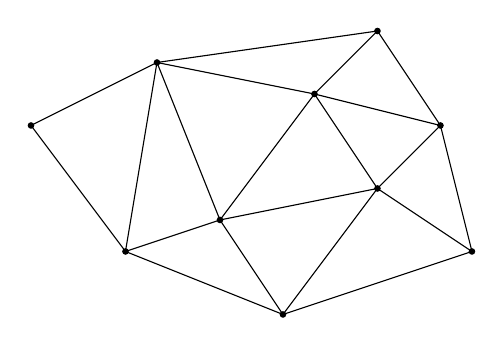
\begin{tikzpicture}[scale=0.4]
		%\draw [<->,thick] (0,10) node (yaxis) [left] {}
		%|- (15,0) node (xaxis) [below] {};
		%centroids
		\fill ( 2, 7) circle (3pt);
		\fill ( 5, 3) circle (3pt);
		\fill ( 6, 9) circle (3pt);
		\fill ( 8, 4) circle (3pt);
		\fill (10, 1) circle (3pt);
		\fill (11, 8) circle (3pt);
		\fill (13, 5) circle (3pt);
		\fill (13,10) circle (3pt);
		\fill (15, 7) circle (3pt);
		\fill (16, 3) circle (3pt);
		
		
		\draw [-] ( 2,7) -- ( 6,9);
		\draw [-] ( 6,9) -- ( 5,3);
		\draw [-] ( 5,3) -- ( 2,7);
		\draw [-] ( 6,9) -- ( 8,4);
		\draw [-] (10,1) -- ( 8,4);
		\draw [-] ( 5,3) -- (10,1);
		\draw [-] ( 8,4) -- ( 5,3);
		\draw [-] ( 8,4) -- (11,8);
		\draw [-] (11,8) -- (6,9);
		\draw [-] ( 6,9) -- (13,10);
		\draw [-] (11,8) -- (13,10);
		\draw [-] (15,7) -- (13,10);
		\draw [-] (16,3) -- (15,7);
		\draw [-] (16,3) -- (10,1);
		\draw [-] (16,3) -- (13,5);
		\draw [-] (13,5) -- (15,7);
		\draw [-] (13,5) -- (10,1);
		\draw [-] (13,5) -- (8,4);
		\draw [-] (13,5) -- (11,8);
		\draw [-] (15,7) -- (11,8);
		\end{tikzpicture}
	\end{center}
	\caption{Example of a Delaunay Triangulation}
	\label{fig:dt1}
\end{figure}
\noindent
More importantly, the Delaunay triangulation of a set of points is the dual graph of its Voronoi Diagram. The edges of the Voronoi diagram, are the line segments connecting the circumcentres of the Delaunay triangles. When overlapped, the duality becomes more obvious. Figure \ref{fig:dt_vd} shows the overlapping of the Voronoi diagram in \ref{fig:vd1} and the Delaunay  triangulation in \ref{fig:dt1}. The Delaunay edges, in black, connect the points at the centre of the Voronoi cells, with edges in red, to their neighbours.
\begin{figure}[H]
	\begin{center}
		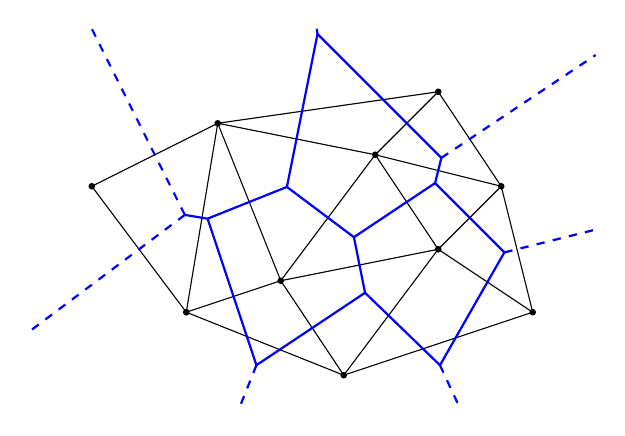
\begin{tikzpicture}[scale=0.4]
		%\draw [<->,thick] (0,10) node (yaxis) [left] {}
		%|- (15,0) node (xaxis) [below] {};
		%centroids
		\fill ( 2, 7) circle (3pt);
		\fill ( 5, 3) circle (3pt);
		\fill ( 6, 9) circle (3pt);
		\fill ( 8, 4) circle (3pt);
		\fill (10, 1) circle (3pt);
		\fill (11, 8) circle (3pt);
		\fill (13, 5) circle (3pt);
		\fill (13,10) circle (3pt);
		\fill (15, 7) circle (3pt);
		\fill (16, 3) circle (3pt);
		
		%DELAUNAY
		\draw [-] ( 2,7) -- ( 6,9);
		\draw [-] ( 6,9) -- ( 5,3);
		\draw [-] ( 5,3) -- ( 2,7);
		\draw [-] ( 6,9) -- ( 8,4);
		\draw [-] (10,1) -- ( 8,4);
		\draw [-] ( 5,3) -- (10,1);
		\draw [-] ( 8,4) -- ( 5,3);
		\draw [-] ( 8,4) -- (11,8);
		\draw [-] (11,8) -- (6,9);
		\draw [-] ( 6,9) -- (13,10);
		\draw [-] (11,8) -- (13,10);
		\draw [-] (15,7) -- (13,10);
		\draw [-] (16,3) -- (15,7);
		\draw [-] (16,3) -- (10,1);
		\draw [-] (16,3) -- (13,5);
		\draw [-] (13,5) -- (15,7);
		\draw [-] (13,5) -- (10,1);
		\draw [-] (13,5) -- (8,4);
		\draw [-] (13,5) -- (11,8);
		\draw [-] (15,7) -- (11,8);
		
		%VORONOI		
		\draw [-,blue,thick] ( 5.6764, 5.9706) -- ( 4.9545, 6.0909);
		\draw [-,blue,thick] ( 5.6764, 5.9706) -- ( 8.1956, 6.9783);
		\draw [-,blue,thick] (10.3235, 5.3824) -- ( 8.1956, 6.9783);
		\draw [-,blue,thick] (10.3235, 5.3824) -- (10.6765, 3.6176);
		\draw [-,blue,thick] ( 7.2272, 1.3182) -- (10.6765, 3.6176);
		\draw [-,blue,thick] ( 7.2272, 1.3182) -- ( 5.6764, 5.9706);
		\draw [-,blue,thick] (13.0556, 1.3182) -- (10.6765, 3.6176);
		\draw [-,blue,thick] (13.0556, 1.3182) -- (15.1000, 4.9000);
		\draw [-,blue,thick] (12.9000, 7.1000) -- (15.1000, 4.9000);
		\draw [-,blue,thick] (12.9000, 7.1000) -- (10.3235, 5.3824);
		\draw [-,blue,thick] (12.9000, 7.1000) -- (13.1000, 7.9000);
		\draw [-,blue,thick] ( 9.1667,11.8333) -- (13.1000, 7.9000);
		\draw [-,blue,thick] ( 9.1667,11.8333) -- ( 8.1956, 6.9783);
		
		\draw [-,blue,thick,dashed] ( 4.9545, 6.0909) -- (	2.0000,12.0000);
		\draw [-,blue,thick,dashed] ( 4.9545, 6.0909) -- (	0.0000,	2.3750);
		\draw [-,blue,thick,dashed] ( 7.2272, 1.3182) -- (	6.7000, 0.0000);
		\draw [-,blue,thick,dashed] (13.0556, 1.3182) -- (13.6667, 0.0000);
		\draw [-,blue,thick,dashed] (15.1000, 4.9000) -- (18.0000, 5.6250);
		\draw [-,blue,thick,dashed] (13.1000, 7.9000) -- (18.0000,11.1667);
		\draw [-,blue,thick,dashed] ( 9.1667,11.8333) -- ( 9.1429,12.0000);
		
		\end{tikzpicture}
	\end{center}
	\caption{Overlap of a Voronoi Diagram and its Delaunay Triangulation}
	\label{fig:dt_vd}
\end{figure}
\noindent
Unlike its counterpart, the Delaunay is much simpler to build incrementally. It is also easier to work with, whilst still providing most of the Voronoi diagram's properties, including the ability to calculate both point location and nearest neighbour searches.
\subsubsection{Greedy Routing}
\label{r:gr}
\paragraph{}
In order to quickly calculate the nearest neighbour to a point in a set, one can make use of the Delaunay triangulation.\\
Consider a triangulation $\mathcal{T}$. In order to find the closest vertex in $\mathcal{T}$ to a new point $p$, we must start at an arbitrary vertex of $\mathcal{T}$, $v$, and find a neighbour $u$ of $v$ whose distance to $p$ is smaller than the distance between $p$ and $v$. Repeat the process for $u$ and its neighbours. When we reach a point $w$ such that no neighbours of $w$ are closer to $p$ than $w$ is, we have found the closest point to $p$ in $\mathcal{T}$.
\begin{figure}[H]
	\begin{center}
		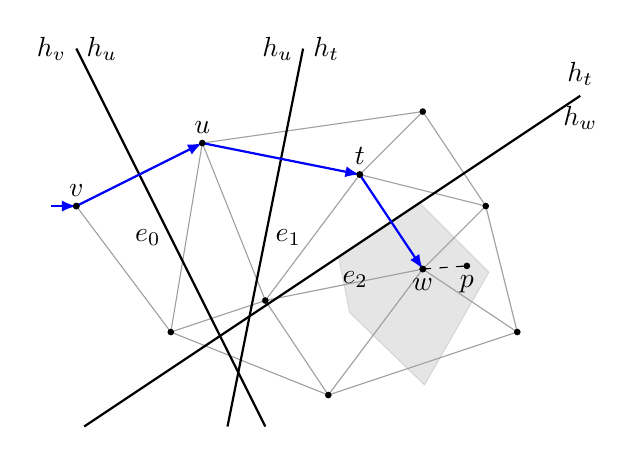
\begin{tikzpicture}[scale=0.4]
		%\draw [<->,thick] (0,10) node (yaxis) [left] {}
		%|- (15,0) node (xaxis) [below] {};
		
		%VORONOI
%		\draw [-,gray!50] ( 5.6764, 5.9706) -- ( 4.9545, 6.0909);
%		\draw [-,gray!50] ( 5.6764, 5.9706) -- ( 8.1956, 6.9783);
%		\draw [-,gray!50] (10.3235, 5.3824) -- ( 8.1956, 6.9783);
%		\draw [-,gray!50] (10.3235, 5.3824) -- (10.6765, 3.6176);
%		\draw [-,gray!50] ( 7.2272, 1.3182) -- (10.6765, 3.6176);
%		\draw [-,gray!50] ( 7.2272, 1.3182) -- ( 5.6764, 5.9706);
%		\draw [-,gray!50] (13.0556, 1.3182) -- (10.6765, 3.6176);
%		\draw [-,gray!50] (13.0556, 1.3182) -- (15.1000, 4.9000);
%		\draw [-,gray!50] (12.9000, 7.1000) -- (15.1000, 4.9000);
%		\draw [-,gray!50] (12.9000, 7.1000) -- (10.3235, 5.3824);
%		\draw [-,gray!50] (12.9000, 7.1000) -- (13.1000, 7.9000);
%		\draw [-,gray!50] ( 9.1667,11.8333) -- (13.1000, 7.9000);
%		%\draw [-,gray!50] ( 9.1667,11.8333) -- ( 8.1956, 6.9783);
%		%VORONOI EXTENDED
%		\draw [-,gray!50] ( 4.9545, 6.0909) -- (2 , 12);
%		\draw [-,gray!50] ( 4.9545, 6.0909) -- (0, 2.375);
%		\draw [-,gray!50] ( 7.2272, 1.3182) -- ( 6.7, 0);
%		\draw [-,gray!50] (13.0556, 1.3182) -- (13.6667, 0);
%		\draw [-,gray!50] (15.1000, 4.9000) -- (18, 5.625);
%		\draw [-,gray!50] (13.1000, 7.9000) -- (18, 11.1667);
%		\draw [-,gray!50] ( 9.1667,11.8333) -- ( 9.1429, 12);
		
		\filldraw[fill=black, opacity=0.1] 	(10.3235, 5.3824) -- (10.6765, 3.6176) --
											(13.0556, 1.3182) -- (15.1000, 4.9000) --
											(12.9000, 7.1000) -- cycle;
		
		%DELAUNAY
		\draw [-,gray!75] ( 2,7) -- ( 6,9);
		\draw [-,gray!75] ( 6,9) -- ( 5,3);
		\draw [-,gray!75] ( 5,3) -- ( 2,7);
		\draw [-,gray!75] ( 6,9) -- ( 8,4);
		\draw [-,gray!75] (10,1) -- ( 8,4);
		\draw [-,gray!75] ( 5,3) -- (10,1);
		\draw [-,gray!75] ( 8,4) -- ( 5,3);
		\draw [-,gray!75] ( 8,4) -- (11,8);
		\draw [-,gray!75] (11,8) -- (6,9);
		\draw [-,gray!75] ( 6,9) -- (13,10);
		\draw [-,gray!75] (11,8) -- (13,10);
		\draw [-,gray!75] (15,7) -- (13,10);
		\draw [-,gray!75] (16,3) -- (15,7);
		\draw [-,gray!75] (16,3) -- (10,1);
		\draw [-,gray!75] (16,3) -- (13,5);
		\draw [-,gray!75] (13,5) -- (15,7);
		\draw [-,gray!75] (13,5) -- (10,1);
		\draw [-,gray!75] (13,5) -- (8,4);
		\draw [-,gray!75] (13,5) -- (11,8);
		\draw [-,gray!75] (15,7) -- (11,8);
		
		
		%POINTS
		
		\fill ( 2, 7) circle (3pt);
		\fill ( 5, 3) circle (3pt);
		\fill ( 8, 4) circle (3pt);
		\fill (10, 1) circle (3pt);
		\fill (11, 8) circle (3pt);
		\fill (13, 5) circle (3pt);
		\fill (13,10) circle (3pt);
		\fill (15, 7) circle (3pt);
		\fill (16, 3) circle (3pt);
		
		%EDGE E
		\draw [-,thick] ( 8,0)		-- node[left]{$e_0$} ( 2, 12)	node[left]		{$h_v$} node[right]{$h_u$};
		\draw [-,thick] ( 6.8,0)	-- node[right]{$e_1$} (9.2,12)	node[left] 		{$h_u$} node[right]{$h_t$};
		\draw [-,thick] ( 2.25,0)	-- node[below right]{$e_2$} (18,10.5)	node[above]{$h_t$} node[below]{$h_w$};
		
		
		\draw [-,dashed]( 13,5) -- ( 14.4, 5.1);
		\draw [->,>=latex,thick,blue]( 1.2,7) -- (  2,7);
		\draw [->,>=latex,thick,blue]( 2,7) -- (  6,9);
		\draw [->,>=latex,thick,blue]( 6,9) -- ( 11, 8);
		\draw [->,>=latex,thick,blue](11,8) -- ( 13, 5);
		\fill (14.4, 5.1) circle (3pt) node[anchor=north]{$p$};
		\fill ( 2, 7)     circle (3pt) node[anchor=south]{$v$};
		\fill ( 6, 9)     circle (3pt) node[anchor=south]{$u$};
		\fill (11, 8)     circle (3pt) node[anchor=south]{$t$};
		\fill (13, 5)     circle (3pt) node[anchor=north]{$w$};
		
		\end{tikzpicture}
	\end{center}
\end{figure}
\begin{theorem}
There is no point set whose Delaunay triangulation defeats the greedy routing algorithm.
\begin{proof}
For every vertex $v$ in a triangulation $\mathcal{T}$, let the perpendicular bisector of the line segment defined by $v$ and $u$ be called $e$ if there is at least one neighbour of $v$, $u$ closer to $p$ than $v$ is. The line $e$ intersects the line segment $(v,p)$ and divides the plane in two open half planes: $h_v$ and $h_u$. Note that the half plane $h_u$ contains $p$.\\
Delaunay edges connect the Voronoi neighbours and their bisectors define the edges of the Voronoi cells, which are convex polygons.\\
Repeating the process recursively for $u$, if a point $w$ is found, whose neighbourhood contains no points closer to $p$ than itself, then $p$ is contained within all possible open half planes containing $w$, defined by $w$ and all its neighbours. Point $p$ is then by definition located in point $w$'s Voronoi cell. This means that $w$ is the point in $\mathcal{T}$ closest to $p$.
\end{proof}
\end{theorem}
\subsubsection{Line Walking}
\paragraph{}
Another point location algorithm to consider is the line walking algorithm. This algorithm finds a triangle $t$ in a triangulation $\mathcal{T}$ that contains a given point $v$. \\
Starting at any triangle $s$, with the geometrical centre $m$, if point $v$ is not contained in $s$, then the line segment $(v,m)$ intersects a finite set of triangles.  
The line segment $(v,m)$ intersects two edges of each triangle in this set, with the exception of $s$ and $t$ where $(v,m)$ only intersects one edge each. 
By iterating through each triangle choosing the neighbour that contains the next edge that intersects $(v,m)$, triangle $t$ can be found in $\mathcal{O}(n)$ time.\\
This algorithm was described by \citet{walking}, and is ilustrated in Figure \ref*{fig:wk1}.
\begin{figure}[H]
	\begin{center}
		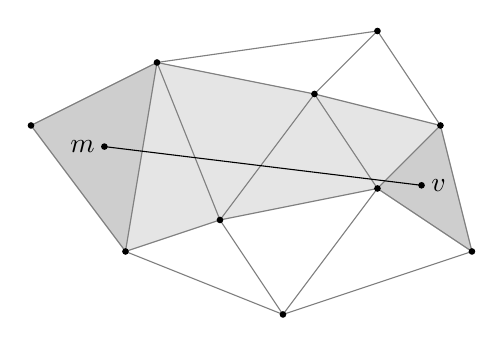
\begin{tikzpicture}[scale=0.4]
		%\draw [<->,thick] (0,10) node (yaxis) [left] {}
		%|- (15,0) node (xaxis) [below] {};
		
		\filldraw[fill=black, opacity=0.1] 	(2,7) -- (6,9) -- 
											(11,8) -- (15,7) -- 
											(16,3) -- (13,5) --
											(8,4) -- (5,3) --
											cycle;
		
		\filldraw[fill=black, opacity=0.1] 	(2,7) -- (6,9) -- (5,3) --
											cycle;
											
		\filldraw[fill=black, opacity=0.1] 	(15,7) -- (13,5) -- (16,3) --
													cycle;
		
		
		
		\draw [-,gray] ( 2,7) -- ( 6,9);
		\draw [-,gray] ( 6,9) -- ( 5,3);
		\draw [-,gray] ( 5,3) -- ( 2,7);
		\draw [-,gray] ( 6,9) -- ( 8,4);
		\draw [-,gray] (10,1) -- ( 8,4);
		\draw [-,gray] ( 5,3) -- (10,1);
		\draw [-,gray] ( 8,4) -- ( 5,3);
		\draw [-,gray] ( 8,4) -- (11,8);
		\draw [-,gray] (11,8) -- (6,9);
		\draw [-,gray] ( 6,9) -- (13,10);
		\draw [-,gray] (11,8) -- (13,10);
		\draw [-,gray] (15,7) -- (13,10);
		\draw [-,gray] (16,3) -- (15,7);
		\draw [-,gray] (16,3) -- (10,1);
		\draw [-,gray] (16,3) -- (13,5);
		\draw [-,gray] (13,5) -- (15,7);
		\draw [-,gray] (13,5) -- (10,1);
		\draw [-,gray] (13,5) -- (8,4);
		\draw [-,gray] (13,5) -- (11,8);
		\draw [-,gray] (15,7) -- (11,8);
		
		
		%centroids
		\fill ( 2, 7) circle (3pt);
		\fill ( 5, 3) circle (3pt);
		\fill ( 6, 9) circle (3pt);
		\fill ( 8, 4) circle (3pt);
		\fill (10, 1) circle (3pt);
		\fill (11, 8) circle (3pt);
		\fill (13, 5) circle (3pt);
		\fill (13,10) circle (3pt);
		\fill (15, 7) circle (3pt);
		\fill (16, 3) circle (3pt);
		
		
		\draw [-]( 4.33,6.33) -- ( 14.4, 5.1);
		%\draw []( 2,7) -- node[anchor=south]{$t$} ( 6,9);
		\fill ( 4.33,6.33) circle (3pt) node[anchor=east]{$m$};
		\fill (14.4, 5.1) circle (3pt) node[anchor=west]{$v$};
		\end{tikzpicture}
	\end{center}
	\caption{Illustration of the Walking Algorithm}
	\label{fig:wk1}
\end{figure}
\subsubsection{Construction}
\label{sect:dtconst}
\paragraph{}
There are many algorithms to construct a Delaunay triangulation. 
The particular conditions of our approach to the coverage problem impose some restrictions to the choice of the algorithm to use.\\
In order to implement an incremental branch and bound approach, our triangulation algorithm has to not only be efficient, but also to be able to be done incrementally. The Bowyer-Watson algorithm allows us to do both.\\
Starting with a valid Delaunay triangulation $\mathcal{T}$, we find a triangle $t = \bigtriangleup_{abc}$ that contains the vertex to insert $v$ using a point location algorithm, such as the walking algorithm. We then use algorithm \ref{alg:bowyer}:
\begin{algorithm}[H]
    \caption{Bowyer-Watson Algorithm}
    \begin{algorithmic}[1]
        \Procedure {InsertVertex}{$v,a,b,c$}
            \State $\text{DeleteTriangle}(a,b,c)$
            \State $\text{DigCavity}(v,a,b)$
            \State $\text{DigCavity}(v,b,c)$
            \State $\text{DigCavity}(v,c,a)$
        \EndProcedure
    \end{algorithmic}
    
    \begin{algorithmic}[1]
       	\Procedure {DigCavity}{$a,b,c$}
        	\State $d \gets \text{Adjacent}(b,c)$
        	\If {$d \neq \varnothing$}
	        	\If {$\text{inCircle}(a,b,c,d)$}
		        	\State $\text{DeleteTriangle}(w,v,x)$
		        	\State $\text{DigCavity}(a,b,d)$
		        	\State $\text{DigCavity}(a,d,c)$
	        	\Else 
		        	\State$\text{AddTriangle}(a,b,c)$
	        	\EndIf
        	\EndIf
       	\EndProcedure
    \end{algorithmic}
    \label{alg:bowyer}
\end{algorithm}
\noindent 
For inserting $n$ points, this algorithm has an expected time complexity of $\mathcal{O}(n \log n)$.

\subsubsection{Deconstruction}
\paragraph{}
Deconstructing a Delaunay triangulation usually takes an algorithm as complex as the construction. However, since in our case the deconstruction has to be incremental, and the first point to remove from the triangulation is necessarily the last one to be inserted, we can use a much simpler approach. \\
At each step of the construction, all created and removed edges and triangle from the triangulation can be stored in a LIFO structure, or a stack. When the last inserted point is to be removed, recreating the previous state of the triangulation is only a matter of rolling back and retrieving the information from the stack. This also means no geometrical calculations have to be done, and the old edges and triangles are quickly put back in place, with no new memory allocation needed.
\subsubsection{Half-Edge Structure}
\paragraph{}
A useful structure to use when building and managing triangulation meshes is the half-edge structure. The half-edge structure represents one orientation of each edge in the triangulation. This means that for each pair of points ($p_i,p_j$)connected in a triangulation $\mathcal{T}$, there are two directed half-edges: one represents the edge from $p_i$ to $p_j$, and the other represents the opposite face, that connects $p_j$ to $p_i$. They both contain information about the triangle that they are part of. The triangles each of them form with two other half-edges contains both $p_i$ and $p_j$, and are thus, adjacent. The way to tell which triangle is which is by defining the triangles by listing their points in a counter-clockwise order. Figure \ref{fig:hedge} further illustrates the concept of the half-edges.\\
\begin{figure}[!h]
	\begin{center}
		\begin{tikzpicture}[scale=0.9,
		arr/.style={->,>=stealth',thick,black,shorten >=3pt,shorten <=3pt},
		edg/.style={black,shorten >=6pt,shorten <=6pt},
		par/.style={decoration={sl,raise=2pt},decorate}]
		
		\node [fill,circle,inner sep=3pt,label=below right:$a$] (A) at (6,1){};
		\node [fill,circle,inner sep=3pt,label=above: $b$] (B) at (5,5){};
		\node [fill,circle,inner sep=3pt,label=left: $c$] (C) at (1,2){};
		\node [fill,circle,inner sep=3pt,label=above right:$d$] (D) at (9,6){};
		
		\path[->,>=latex]
		(A) edge [arr,par](B)
		(B) edge [arr,par](C)
		(C) edge [arr,par](B)
		(C) edge [arr,par](A)
		(A) edge [arr,par](C)
		
		(B) edge [arr,par](A)
		(A) edge [arr,par](D)
		(D) edge [arr,par](B)
		(D) edge [arr,par](A)
		(B) edge [arr,par](D);
		\draw [arr,par,dashed,gray] (B) -- (3,7);
		\draw [arr,par,dashed,gray] (3,7) -- (B);
		
		\draw [arr,par,dashed,gray] (C) -- (0.5,0);
		\draw [arr,par,dashed,gray] (0.5,0) -- (C);
		
		\draw [arr,par,dashed,gray] (C) -- (0,4);
		\draw [arr,par,dashed,gray] (0,4) -- (C);
		
		\draw [arr,par,dashed,gray] (A) -- (5,0);
		\draw [arr,par,dashed,gray] (5,0) -- (A);
		
		\draw [arr,par,dashed,gray] (A) -- (10,2);
		\draw [arr,par,dashed,gray] (10,2) -- (A);
		
		\draw [arr,par,dashed,gray] (D) -- (10,4);
		\draw [arr,par,dashed,gray] (10,4) -- (D);
		
		\draw [arr,par,dashed,gray] (D) -- (7,7);
		\draw [arr,par,dashed,gray] (7,7) -- (D);

		
%		\path[-,color=gray]
%		(A) edge (B)
%		(B) edge (C)
%		(C) edge (A)
%		(A) edge (D)
%		(D) edge (B)		
%		;
		\end{tikzpicture}
	\end{center}
	\caption{Illustration of the Half-Edge Structure}
	\label{fig:hedge}
\end{figure}
This structure makes it easier to store the changes to the triangulation in each step, since they contain the information about the triangles themselves. This means that only the half edges need to be stored in the stack, with no need to deal with the triangles directly.
The half-edge structure helps to obtain the triangulation neighbours for any vertex $v$, since these are all the end points to the half-edges starting at $v$, which is useful when implementing the greedy routing algorithm described in \ref{r:gr}. 
\subsection{Hilbert Curves}
\paragraph{}
Most of the point location algorithms aforementioned have linear time complexity, and most of the worst case scenarios include searching across the plane. These occur when the starting search position is random and does not make use of the spatial organisation of the data. In order to fully take advantage of these approaches, the points should be sorted is such a way that minimizes the distance between consecutive point such as a Hilbert curve. \\
Hilbert curves are a kind of fractal space-filling curves that generally minimize the Euclidean distance between points close on the curve.\\
True Hilbert curves map a 2-dimensional space in a 1-dimension line. This line has an infinite length, which makes mapping 2-dimensional points to it infeasible. Instead, discrete approximations are used. Since the true curve is fractal, the approximations are defined by the number of fractal steps it takes in order to reach them. Figure \ref*{fig:hilbert} demonstrates the first few orders of approximation:
\begin{figure}[H]
	\begin{center}
		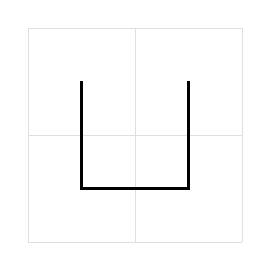
\begin{tikzpicture}[scale=0.17]
		\draw [step=8,gray,very thin,opacity=0.25](0,0) grid(16,16);
		\draw [-,thick] 	(4,12) -- ( 4,4) -- ( 12,4) -- ( 12,12);
		\end{tikzpicture}
		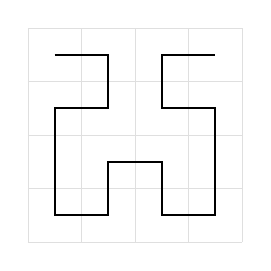
\begin{tikzpicture}[scale=0.17]
		\draw [step=4,gray,very thin,opacity=0.25](0,0) grid(16,16);
		\draw [-,thick]
				 	(2,14) -- ( 6,14) -- (6,10) -- (2,10) -- 
					(2,2)  -- (6,2) -- (6,6) -- (10,6) -- 
					(10,2) -- (14,2) -- (14,10)--(10,10) --
					(10,14) -- (14,14);
		\end{tikzpicture}
		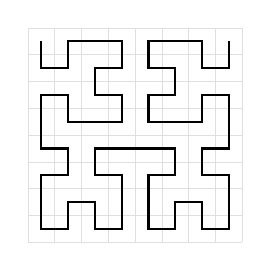
\begin{tikzpicture}[scale=0.17]
		\draw [step=2,gray,very thin,opacity=0.25](0,0) grid(16,16);
		\draw [-,thick] 
					(1,15) 	-- (1,13) 	-- (3,13) 	-- (3,15) 	-- (7,15) 	--
					(7,13) 	-- (5,13) 	-- (5,11)	-- (7,11) 	-- (7,9) 	--
					(3,9) 	-- (3,11)	-- (1,11)	-- (1,7) 	-- (3,7) 	--
					(3,5) 	-- (1,5) 	-- (1,1)	-- (3,1) 	-- (3,3) 	-- 
					(5,3) 	-- (5,1) 	-- (7,1)  	-- (7,5) 	-- (5,5) 	--
					(5,7) 	-- (11,7) 	-- (11,5)  	-- (9,5) 	-- (9,1) 	--
					(11,1)	-- (11,3) 	-- (13,3)  	-- (13,1) 	-- (15,1) 	--
					(15,5) 	-- (13,5) 	-- (13,7)  	-- (15,7) 	-- (15,11)	--
					(13,11)	-- (13,9)  	-- (9,9) 	-- (9,11) 	-- (11,11)	--
					(11,13)	-- (9,13) 	-- (9,15) 	-- (13,15)  -- (13,13) 	--
					(15,13) -- (15,15)
					;
		
		\end{tikzpicture}
		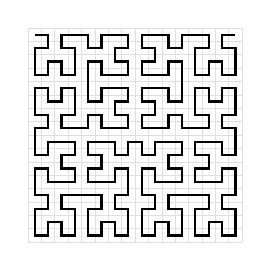
\begin{tikzpicture}[scale=0.17]
		\draw [step=1,gray,very thin,opacity=0.25](0,0) grid(16,16);
		\draw [-,thick] 
				(0.5, 15.5)	-- (1.5, 15.5) 	-- (1.5, 14.5) 	-- (0.5, 14.5) 	-- 
				(0.5, 13.5)	-- (0.5, 12.5) 	-- (1.5, 12.5) 	-- (1.5, 13.5) 	-- 
				(2.5, 13.5)	-- (2.5, 12.5) 	-- (3.5, 12.5) 	-- (3.5, 13.5) 	-- 
				(3.5, 14.5) -- (2.5, 14.5) 	-- (2.5, 15.5) 	-- (3.5, 15.5) 	-- 
				(4.5, 15.5) -- (4.5, 14.5) 	-- (5.5, 14.5) 	-- (5.5, 15.5) 	-- 
				(6.5, 15.5) -- (7.5, 15.5) 	-- (7.5, 14.5) 	-- (6.5, 14.5) 	-- 
				(6.5, 13.5) -- (7.5, 13.5) 	-- (7.5, 12.5) 	-- (6.5, 12.5) 	-- 
				(5.5, 12.5) -- (5.5, 13.5) 	-- (4.5, 13.5) 	-- (4.5, 12.5) 	-- 
				(4.5, 11.5) -- (4.5, 10.5) 	-- (5.5, 10.5) 	-- (5.5, 11.5) 	-- 
				(6.5, 11.5) -- (7.5, 11.5) 	-- (7.5, 10.5) 	-- (6.5, 10.5) 	-- 
				(6.5, 9.5) 	-- (7.5, 9.5) 	-- (7.5, 8.5) 	-- (6.5, 8.5) 	-- 
				(5.5, 8.5) 	-- (5.5, 9.5) 	-- (4.5, 9.5) 	-- (4.5, 8.5) 	-- 
				(3.5, 8.5) 	-- (2.5, 8.5) 	-- (2.5, 9.5) 	-- (3.5, 9.5) 	-- 
				(3.5, 10.5) -- (3.5, 11.5) 	-- (2.5, 11.5) 	-- (2.5, 10.5) 	-- 
				(1.5, 10.5) -- (1.5, 11.5) 	-- (0.5, 11.5) 	-- (0.5, 10.5) 	-- 
				(0.5, 9.5) 	-- (1.5, 9.5)	-- (1.5, 8.5) 	-- (0.5, 8.5) 	-- 
				(0.5, 7.5) 	-- (0.5, 6.5) 	-- (1.5, 6.5) 	-- (1.5, 7.5) 	-- 
				(2.5, 7.5) 	-- (3.5, 7.5) 	-- (3.5, 6.5) 	-- (2.5, 6.5) 	-- 
				(2.5, 5.5) 	-- (3.5, 5.5) 	-- (3.5, 4.5) 	-- (2.5, 4.5) 	-- 
				(1.5, 4.5) 	-- (1.5, 5.5) 	-- (0.5, 5.5) 	-- (0.5, 4.5) 	-- 
				(0.5, 3.5) 	-- (1.5, 3.5) 	-- (1.5, 2.5) 	-- (0.5, 2.5) 	-- 
				(0.5, 1.5) 	-- (0.5, 0.5) 	-- (1.5, 0.5)	-- (1.5, 1.5) 	-- 
				(2.5, 1.5) 	-- (2.5, 0.5) 	-- (3.5, 0.5) 	-- (3.5, 1.5) 	-- 
				(3.5, 2.5) 	-- (2.5, 2.5) 	-- (2.5, 3.5) 	-- (3.5, 3.5) 	-- 
				(4.5, 3.5) 	-- (5.5, 3.5) 	-- (5.5, 2.5) 	-- (4.5, 2.5) 	-- 
				(4.5, 1.5) 	-- (4.5, 0.5) 	-- (5.5, 0.5) 	-- (5.5, 1.5) 	-- 
				(6.5, 1.5) 	-- (6.5, 0.5) 	-- (7.5, 0.5) 	-- (7.5, 1.5) 	-- 
				(7.5, 2.5) 	-- (6.5, 2.5) 	-- (6.5, 3.5) 	-- (7.5, 3.5) 	-- 
				(7.5, 4.5) 	-- (7.5, 5.5) 	-- (6.5, 5.5) 	-- (6.5, 4.5) 	-- 
				(5.5, 4.5) 	-- (4.5, 4.5) 	-- (4.5, 5.5) 	-- (5.5, 5.5) 	-- 
				(5.5, 6.5) 	-- (4.5, 6.5) 	-- (4.5, 7.5) 	-- (5.5, 7.5) 	-- 
				(6.5, 7.5) 	-- (6.5, 6.5) 	-- (7.5, 6.5) 	-- (7.5, 7.5) 	-- 
				(8.5, 7.5) 	-- (8.5, 6.5) 	-- (9.5, 6.5) 	-- (9.5, 7.5) 	-- 
				(10.5, 7.5) -- (11.5, 7.5) 	-- (11.5, 6.5) 	-- (10.5, 6.5) 	-- 
				(10.5, 5.5)	-- (11.5, 5.5) 	-- (11.5, 4.5) 	-- (10.5, 4.5) 	-- 
				(9.5, 4.5) 	-- (9.5, 5.5) 	-- (8.5, 5.5) 	-- (8.5, 4.5) 	-- 
				(8.5, 3.5) 	-- (9.5, 3.5) 	-- (9.5, 2.5) 	-- (8.5, 2.5) 	-- 
				(8.5, 1.5) 	-- (8.5, 0.5) 	-- (9.5, 0.5) 	-- (9.5, 1.5) 	-- 
				(10.5, 1.5) -- (10.5, 0.5) 	-- (11.5, 0.5) 	-- (11.5, 1.5) 	-- 
				(11.5, 2.5) -- (10.5, 2.5) 	-- (10.5, 3.5) 	-- (11.5, 3.5) 	-- 
				(12.5, 3.5) -- (13.5, 3.5)	-- (13.5, 2.5) 	-- (12.5, 2.5) 	-- 
				(12.5, 1.5) -- (12.5, 0.5) 	-- (13.5, 0.5) 	-- (13.5, 1.5) 	-- 
				(14.5, 1.5) -- (14.5, 0.5) 	-- (15.5, 0.5) 	-- (15.5, 1.5) 	-- 
				(15.5, 2.5) -- (14.5, 2.5) 	-- (14.5, 3.5) 	-- (15.5, 3.5) 	-- 
				(15.5, 4.5) -- (15.5, 5.5) 	-- (14.5, 5.5) 	-- (14.5, 4.5) 	-- 
				(13.5, 4.5) -- (12.5, 4.5) 	-- (12.5, 5.5) 	-- (13.5, 5.5) 	-- 
				(13.5, 6.5) -- (12.5, 6.5) 	-- (12.5, 7.5) 	-- (13.5, 7.5) 	-- 
				(14.5, 7.5) -- (14.5, 6.5) 	-- (15.5, 6.5) 	-- (15.5, 7.5) 	-- 
				(15.5, 8.5) -- (14.5, 8.5) 	-- (14.5, 9.5) 	-- (15.5, 9.5) 	-- 
				(15.5, 10.5)-- (15.5, 11.5)	-- (14.5, 11.5)	-- (14.5, 10.5)	-- 
				(13.5, 10.5)-- (13.5, 11.5)	-- (12.5, 11.5)	-- (12.5, 10.5)	--
				(12.5, 9.5)	-- (13.5, 9.5) 	-- (13.5, 8.5)	-- (12.5, 8.5) 	-- 
				(11.5, 8.5) -- (11.5, 9.5) 	-- (10.5, 9.5) 	-- (10.5, 8.5) 	-- 
				(9.5, 8.5) 	-- (8.5, 8.5) 	-- (8.5, 9.5) 	-- (9.5, 9.5) 	--
				(9.5, 10.5) -- (8.5, 10.5) 	-- (8.5, 11.5) 	-- (9.5, 11.5) 	-- 
				(10.5, 11.5)-- (10.5, 10.5)	-- (11.5, 10.5)	-- (11.5, 11.5)	-- 
				(11.5, 12.5)-- (11.5, 13.5)	-- (10.5, 13.5)	-- (10.5, 12.5)	-- 
				(9.5, 12.5) -- (8.5, 12.5) 	-- (8.5, 13.5) 	-- (9.5, 13.5) 	-- 
				(9.5, 14.5) -- (8.5, 14.5) 	-- (8.5, 15.5) 	-- (9.5, 15.5) 	--
				(10.5, 15.5)-- (10.5, 14.5)	-- (11.5, 14.5)	-- (11.5, 15.5)	-- 
				(12.5, 15.5)-- (13.5, 15.5)	-- (13.5, 14.5)	-- (12.5, 14.5)	-- 
				(12.5, 13.5)-- (12.5, 12.5)	-- (13.5, 12.5)	-- (13.5, 13.5)	--
				(14.5, 13.5)-- (14.5, 12.5)	-- (15.5, 12.5)	-- (15.5, 13.5)	--
				(15.5, 14.5)-- (14.5, 14.5)	-- (14.5, 15.5)	-- (15.5, 15.5)
		;		
		\end{tikzpicture}
		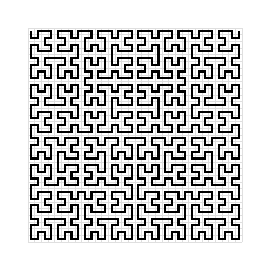
\begin{tikzpicture}[scale=0.17]
		\draw [step=0.5,gray,very thin,opacity=0.25](0,0) grid(16,16);
		\draw [-,thick]
					(15.75,15.75)	--(15.75, 15.25) 	-- (15.25, 15.25) 	-- (15.25, 15.75) 	-- (14.75, 15.75) 	-- (14.25, 15.75) 	-- (14.25, 15.25) 	-- (14.75, 15.25) 	-- (14.75, 14.75) 	-- (14.25, 14.75) 	-- (14.25, 14.25) 	-- (14.75, 14.25) 	-- (15.25, 14.25) 	-- (15.25, 14.75) 	-- (15.75, 14.75) 	-- (15.75, 14.25) 	-- (15.75, 13.75) 	-- (15.25, 13.75) 	-- (15.25, 13.25) 	-- (15.75, 13.25) 	-- (15.75, 12.75) 	-- (15.75, 12.25) 	-- (15.25, 12.25) 	-- (15.25, 12.75) 	-- (14.75, 12.75) 	-- (14.75, 12.25) 	-- (14.25, 12.25) 	-- (14.25, 12.75) 	-- (14.25, 13.25) 	-- (14.75, 13.25) 	-- (14.75, 13.75) 	-- (14.25, 13.75) 	-- (13.75, 13.75) 	-- (13.25, 13.75) 	-- (13.25, 13.25) 	-- (13.75, 13.25) 	-- (13.75, 12.75) 	-- (13.75, 12.25) 	-- (13.25, 12.25) 	-- (13.25, 12.75) 	-- (12.75, 12.75) 	-- (12.75, 12.25) 	-- (12.25, 12.25) 	-- (12.25, 12.75) 	-- (12.25, 13.25) 	-- (12.75, 13.25) 	-- (12.75, 13.75) 	-- (12.25, 13.75) 	-- (12.25, 14.25) 	-- (12.25, 14.75) 	-- (12.75, 14.75) 	-- (12.75, 14.25) 	-- (13.25, 14.25) 	-- (13.75, 14.25) 	-- (13.75, 14.75) 	-- (13.25, 14.75) 	-- (13.25, 15.25) 	-- (13.75, 15.25) 	-- (13.75, 15.75) 	-- (13.25, 15.75) 	-- (12.75, 15.75) 	-- (12.75, 15.25) 	-- (12.25, 15.25) 	-- (12.25, 15.75) 	-- (11.75, 15.75) 	-- (11.25, 15.75) 	-- (11.25, 15.25) 	-- (11.75, 15.25) 	-- (11.75, 14.75) 	-- (11.75, 14.25) 	-- (11.25, 14.25) 	-- (11.25, 14.75) 	-- (10.75, 14.75) 	-- (10.75, 14.25) 	-- (10.25, 14.25) 	-- (10.25, 14.75) 	-- (10.25, 15.25) 	-- (10.75, 15.25) 	-- (10.75, 15.75) 	-- (10.25, 15.75) 	-- (9.75, 15.75) 	-- (9.75, 15.25) 	-- (9.25, 15.25) 	-- (9.25, 15.75) 	-- (8.75, 15.75) 	-- (8.25, 15.75) 	-- (8.25, 15.25) 	-- (8.75, 15.25) 	-- (8.75, 14.75) 	-- (8.25, 14.75) 	-- (8.25, 14.25) 	-- (8.75, 14.25) 	-- (9.25, 14.25) 	-- (9.25, 14.75) 	-- (9.75, 14.75) 	-- (9.75, 14.25) 	-- (9.75, 13.75) 	-- (9.75, 13.25) 	-- (9.25, 13.25) 	-- (9.25, 13.75) 	-- (8.75, 13.75) 	-- (8.25, 13.75) 	-- (8.25, 13.25) 	-- (8.75, 13.25) 	-- (8.75, 12.75) 	-- (8.25, 12.75) 	-- (8.25, 12.25) 	-- (8.75, 12.25) 	-- (9.25, 12.25) 	-- (9.25, 12.75) 	-- (9.75, 12.75) 	-- (9.75, 12.25) 	-- (10.25, 12.25) 	-- (10.75, 12.25) 	-- (10.75, 12.75) 	-- (10.25, 12.75) 	-- (10.25, 13.25) 	-- (10.25, 13.75) 	-- (10.75, 13.75) 	-- (10.75, 13.25) 	-- (11.25, 13.25) 	-- (11.25, 13.75) 	-- (11.75, 13.75) 	-- (11.75, 13.25) 	-- (11.75, 12.75) 	-- (11.25, 12.75) 	-- (11.25, 12.25) 	-- (11.75, 12.25) 	-- (11.75, 11.75) 	-- (11.25, 11.75) 	-- (11.25, 11.25) 	-- (11.75, 11.25) 	-- (11.75, 10.75) 	-- (11.75, 10.25) 	-- (11.25, 10.25) 	-- (11.25, 10.75) 	-- (10.75, 10.75) 	-- (10.75, 10.25) 	-- (10.25, 10.25) 	-- (10.25, 10.75) 	-- (10.25, 11.25) 	-- (10.75, 11.25) 	-- (10.75, 11.75) 	-- (10.25, 11.75) 	-- (9.75, 11.75) 	-- (9.75, 11.25) 	-- (9.25, 11.25) 	-- (9.25, 11.75) 	-- (8.75, 11.75) 	-- (8.25, 11.75) 	-- (8.25, 11.25) 	-- (8.75, 11.25) 	-- (8.75, 10.75) 	-- (8.25, 10.75) 	-- (8.25, 10.25) 	-- (8.75, 10.25) 	-- (9.25, 10.25) 	-- (9.25, 10.75) 	-- (9.75, 10.75) 	-- (9.75, 10.25) 	-- (9.75, 9.75) 	-- (9.75, 9.25) 	-- (9.25, 9.25) 	-- (9.25, 9.75) 	-- (8.75, 9.75) 	-- (8.25, 9.75) 	-- (8.25, 9.25) 	-- (8.75, 9.25) 	-- (8.75, 8.75) 	-- (8.25, 8.75) 	-- (8.25, 8.25) 	-- (8.75, 8.25) 	-- (9.25, 8.25) 	-- (9.25, 8.75) 	-- (9.75, 8.75) 	-- (9.75, 8.25) 	-- (10.25, 8.25) 	-- (10.75, 8.25) 	-- (10.75, 8.75) 	-- (10.25, 8.75) 	-- (10.25, 9.25) 	-- (10.25, 9.75) 	-- (10.75, 9.75) 	-- (10.75, 9.25) 	-- (11.25, 9.25) 	-- (11.25, 9.75) 	-- (11.75, 9.75) 	-- (11.75, 9.25) 	-- (11.75, 8.75) 	-- (11.25, 8.75) 	-- (11.25, 8.25) 	-- (11.75, 8.25) 	-- (12.25, 8.25) 	-- (12.25, 8.75) 	-- (12.75, 8.75) 	-- (12.75, 8.25) 	-- (13.25, 8.25) 	-- (13.75, 8.25) 	-- (13.75, 8.75) 	-- (13.25, 8.75) 	-- (13.25, 9.25) 	-- (13.75, 9.25) 	-- (13.75, 9.75) 	-- (13.25, 9.75) 	-- (12.75, 9.75) 	-- (12.75, 9.25) 	-- (12.25, 9.25) 	-- (12.25, 9.75) 	-- (12.25, 10.25) 	-- (12.75, 10.25) 	-- (12.75, 10.75) 	-- (12.25, 10.75) 	-- (12.25, 11.25) 	-- (12.25, 11.75) 	-- (12.75, 11.75) 	-- (12.75, 11.25) 	-- (13.25, 11.25) 	-- (13.25, 11.75) 	-- (13.75, 11.75) 	-- (13.75, 11.25) 	-- (13.75, 10.75) 	-- (13.25, 10.75) 	-- (13.25, 10.25) 	-- (13.75, 10.25) 	-- (14.25, 10.25) 	-- (14.75, 10.25) 	-- (14.75, 10.75) 	-- (14.25, 10.75) 	-- (14.25, 11.25) 	-- (14.25, 11.75) 	-- (14.75, 11.75) 	-- (14.75, 11.25) 	-- (15.25, 11.25) 	-- (15.25, 11.75) 	-- (15.75, 11.75) 	-- (15.75, 11.25) 	-- (15.75, 10.75) 	-- (15.25, 10.75) 	-- (15.25, 10.25) 	-- (15.75, 10.25) 	-- (15.75, 9.75) 	-- (15.75, 9.25) 	-- (15.25, 9.25) 	-- (15.25, 9.75) 	-- (14.75, 9.75) 	-- (14.25, 9.75) 	-- (14.25, 9.25) 	-- (14.75, 9.25) 	-- (14.75, 8.75) 	-- (14.25, 8.75) 	-- (14.25, 8.25) 	-- (14.75, 8.25) 	-- (15.25, 8.25) 	-- (15.25, 8.75) 	-- (15.75, 8.75) 	-- (15.75, 8.25) 	-- (15.75, 7.75) 	-- (15.25, 7.75) 	-- (15.25, 7.25) 	-- (15.75, 7.25) 	-- (15.75, 6.75) 	-- (15.75, 6.25) 	-- (15.25, 6.25) 	-- (15.25, 6.75) 	-- (14.75, 6.75) 	-- (14.75, 6.25) 	-- (14.25, 6.25) 	-- (14.25, 6.75) 	-- (14.25, 7.25) 	-- (14.75, 7.25) 	-- (14.75, 7.75) 	-- (14.25, 7.75) 	-- (13.75, 7.75) 	-- (13.75, 7.25) 	-- (13.25, 7.25) 	-- (13.25, 7.75) 	-- (12.75, 7.75) 	-- (12.25, 7.75) 	-- (12.25, 7.25) 	-- (12.75, 7.25) 	-- (12.75, 6.75) 	-- (12.25, 6.75) 	-- (12.25, 6.25) 	-- (12.75, 6.25) 	-- (13.25, 6.25) 	-- (13.25, 6.75) 	-- (13.75, 6.75) 	-- (13.75, 6.25) 	-- (13.75, 5.75) 	-- (13.75, 5.25) 	-- (13.25, 5.25) 	-- (13.25, 5.75) 	-- (12.75, 5.75) 	-- (12.25, 5.75) 	-- (12.25, 5.25) 	-- (12.75, 5.25) 	-- (12.75, 4.75) 	-- (12.25, 4.75) 	-- (12.25, 4.25) 	-- (12.75, 4.25) 	-- (13.25, 4.25) 	-- (13.25, 4.75) 	-- (13.75, 4.75) 	-- (13.75, 4.25) 	-- (14.25, 4.25) 	-- (14.75, 4.25) 	-- (14.75, 4.75) 	-- (14.25, 4.75) 	-- (14.25, 5.25) 	-- (14.25, 5.75) 	-- (14.75, 5.75) 	-- (14.75, 5.25) 	-- (15.25, 5.25) 	-- (15.25, 5.75) 	-- (15.75, 5.75) 	-- (15.75, 5.25) 	-- (15.75, 4.75) 	-- (15.25, 4.75) 	-- (15.25, 4.25) 	-- (15.75, 4.25) 	-- (15.75, 3.75) 	-- (15.75, 3.25) 	-- (15.25, 3.25) 	-- (15.25, 3.75) 	-- (14.75, 3.75) 	-- (14.25, 3.75) 	-- (14.25, 3.25) 	-- (14.75, 3.25) 	-- (14.75, 2.75) 	-- (14.25, 2.75) 	-- (14.25, 2.25) 	-- (14.75, 2.25) 	-- (15.25, 2.25) 	-- (15.25, 2.75) 	-- (15.75, 2.75) 	-- (15.75, 2.25) 	-- (15.75, 1.75) 	-- (15.25, 1.75) 	-- (15.25, 1.25) 	-- (15.75, 1.25) 	-- (15.75, 0.75) 	-- (15.75, 0.25) 	-- (15.25, 0.25) 	-- (15.25, 0.75) 	-- (14.75, 0.75) 	-- (14.75, 0.25) 	-- (14.25, 0.25) 	-- (14.25, 0.75) 	-- (14.25, 1.25) 	-- (14.75, 1.25) 	-- (14.75, 1.75) 	-- (14.25, 1.75) 	-- (13.75, 1.75) 	-- (13.25, 1.75) 	-- (13.25, 1.25) 	-- (13.75, 1.25) 	-- (13.75, 0.75) 	-- (13.75, 0.25) 	-- (13.25, 0.25) 	-- (13.25, 0.75) 	-- (12.75, 0.75) 	-- (12.75, 0.25) 	-- (12.25, 0.25) 	-- (12.25, 0.75) 	-- (12.25, 1.25) 	-- (12.75, 1.25) 	-- (12.75, 1.75) 	-- (12.25, 1.75) 	-- (12.25, 2.25) 	-- (12.25, 2.75) 	-- (12.75, 2.75) 	-- (12.75, 2.25) 	-- (13.25, 2.25) 	-- (13.75, 2.25) 	-- (13.75, 2.75) 	-- (13.25, 2.75) 	-- (13.25, 3.25) 	-- (13.75, 3.25) 	-- (13.75, 3.75) 	-- (13.25, 3.75) 	-- (12.75, 3.75) 	-- (12.75, 3.25) 	-- (12.25, 3.25) 	-- (12.25, 3.75) 	-- (11.75, 3.75) 	-- (11.75, 3.25) 	-- (11.25, 3.25) 	-- (11.25, 3.75) 	-- (10.75, 3.75) 	-- (10.25, 3.75) 	-- (10.25, 3.25) 	-- (10.75, 3.25) 	-- (10.75, 2.75) 	-- (10.25, 2.75) 	-- (10.25, 2.25) 	-- (10.75, 2.25) 	-- (11.25, 2.25) 	-- (11.25, 2.75) 	-- (11.75, 2.75) 	-- (11.75, 2.25) 	-- (11.75, 1.75) 	-- (11.25, 1.75) 	-- (11.25, 1.25) 	-- (11.75, 1.25) 	-- (11.75, 0.75) 	-- (11.75, 0.25) 	-- (11.25, 0.25) 	-- (11.25, 0.75) 	-- (10.75, 0.75) 	-- (10.75, 0.25) 	-- (10.25, 0.25) 	-- (10.25, 0.75) 	-- (10.25, 1.25) 	-- (10.75, 1.25) 	-- (10.75, 1.75) 	-- (10.25, 1.75) 	-- (9.75, 1.75) 	-- (9.25, 1.75) 	-- (9.25, 1.25) 	-- (9.75, 1.25) 	-- (9.75, 0.75) 	-- (9.75, 0.25) 	-- (9.25, 0.25) 	-- (9.25, 0.75) 	-- (8.75, 0.75) 	-- (8.75, 0.25) 	-- (8.25, 0.25) 	-- (8.25, 0.75) 	-- (8.25, 1.25) 	-- (8.75, 1.25) 	-- (8.75, 1.75) 	-- (8.25, 1.75) 	-- (8.25, 2.25) 	-- (8.25, 2.75) 	-- (8.75, 2.75) 	-- (8.75, 2.25) 	-- (9.25, 2.25) 	-- (9.75, 2.25) 	-- (9.75, 2.75) 	-- (9.25, 2.75) 	-- (9.25, 3.25) 	-- (9.75, 3.25) 	-- (9.75, 3.75) 	-- (9.25, 3.75) 	-- (8.75, 3.75) 	-- (8.75, 3.25) 	-- (8.25, 3.25) 	-- (8.25, 3.75) 	-- (8.25, 4.25) 	-- (8.75, 4.25) 	-- (8.75, 4.75) 	-- (8.25, 4.75) 	-- (8.25, 5.25) 	-- (8.25, 5.75) 	-- (8.75, 5.75) 	-- (8.75, 5.25) 	-- (9.25, 5.25) 	-- (9.25, 5.75) 	-- (9.75, 5.75) 	-- (9.75, 5.25) 	-- (9.75, 4.75) 	-- (9.25, 4.75) 	-- (9.25, 4.25) 	-- (9.75, 4.25) 	-- (10.25, 4.25) 	-- (10.25, 4.75) 	-- (10.75, 4.75) 	-- (10.75, 4.25) 	-- (11.25, 4.25) 	-- (11.75, 4.25) 	-- (11.75, 4.75) 	-- (11.25, 4.75) 	-- (11.25, 5.25) 	-- (11.75, 5.25) 	-- (11.75, 5.75) 	-- (11.25, 5.75) 	-- (10.75, 5.75) 	-- (10.75, 5.25) 	-- (10.25, 5.25) 	-- (10.25, 5.75) 	-- (10.25, 6.25) 	-- (10.25, 6.75) 	-- (10.75, 6.75) 	-- (10.75, 6.25) 	-- (11.25, 6.25) 	-- (11.75, 6.25) 	-- (11.75, 6.75) 	-- (11.25, 6.75) 	-- (11.25, 7.25) 	-- (11.75, 7.25) 	-- (11.75, 7.75) 	-- (11.25, 7.75) 	-- (10.75, 7.75) 	-- (10.75, 7.25) 	-- (10.25, 7.25) 	-- (10.25, 7.75) 	-- (9.75, 7.75) 	-- (9.25, 7.75) 	-- (9.25, 7.25) 	-- (9.75, 7.25) 	-- (9.75, 6.75) 	-- (9.75, 6.25) 	-- (9.25, 6.25) 	-- (9.25, 6.75) 	-- (8.75, 6.75) 	-- (8.75, 6.25) 	-- (8.25, 6.25) 	-- (8.25, 6.75) 	-- (8.25, 7.25) 	-- (8.75, 7.25) 	-- (8.75, 7.75) 	-- (8.25, 7.75) 	-- (7.75, 7.75) 	-- (7.25, 7.75) 	-- (7.25, 7.25) 	-- (7.75, 7.25) 	-- (7.75, 6.75) 	-- (7.75, 6.25) 	-- (7.25, 6.25) 	-- (7.25, 6.75) 	-- (6.75, 6.75) 	-- (6.75, 6.25) 	-- (6.25, 6.25) 	-- (6.25, 6.75) 	-- (6.25, 7.25) 	-- (6.75, 7.25) 	-- (6.75, 7.75) 	-- (6.25, 7.75) 	-- (5.75, 7.75) 	-- (5.75, 7.25) 	-- (5.25, 7.25) 	-- (5.25, 7.75) 	-- (4.75, 7.75) 	-- (4.25, 7.75) 	-- (4.25, 7.25) 	-- (4.75, 7.25) 	-- (4.75, 6.75) 	-- (4.25, 6.75) 	-- (4.25, 6.25) 	-- (4.75, 6.25) 	-- (5.25, 6.25) 	-- (5.25, 6.75) 	-- (5.75, 6.75) 	-- (5.75, 6.25) 	-- (5.75, 5.75) 	-- (5.75, 5.25) 	-- (5.25, 5.25) 	-- (5.25, 5.75) 	-- (4.75, 5.75) 	-- (4.25, 5.75) 	-- (4.25, 5.25) 	-- (4.75, 5.25) 	-- (4.75, 4.75) 	-- (4.25, 4.75) 	-- (4.25, 4.25) 	-- (4.75, 4.25) 	-- (5.25, 4.25) 	-- (5.25, 4.75) 	-- (5.75, 4.75) 	-- (5.75, 4.25) 	-- (6.25, 4.25) 	-- (6.75, 4.25) 	-- (6.75, 4.75) 	-- (6.25, 4.75) 	-- (6.25, 5.25) 	-- (6.25, 5.75) 	-- (6.75, 5.75) 	-- (6.75, 5.25) 	-- (7.25, 5.25) 	-- (7.25, 5.75) 	-- (7.75, 5.75) 	-- (7.75, 5.25) 	-- (7.75, 4.75) 	-- (7.25, 4.75) 	-- (7.25, 4.25) 	-- (7.75, 4.25) 	-- (7.75, 3.75) 	-- (7.75, 3.25) 	-- (7.25, 3.25) 	-- (7.25, 3.75) 	-- (6.75, 3.75) 	-- (6.25, 3.75) 	-- (6.25, 3.25) 	-- (6.75, 3.25) 	-- (6.75, 2.75) 	-- (6.25, 2.75) 	-- (6.25, 2.25) 	-- (6.75, 2.25) 	-- (7.25, 2.25) 	-- (7.25, 2.75) 	-- (7.75, 2.75) 	-- (7.75, 2.25) 	-- (7.75, 1.75) 	-- (7.25, 1.75) 	-- (7.25, 1.25) 	-- (7.75, 1.25) 	-- (7.75, 0.75) 	-- (7.75, 0.25) 	-- (7.25, 0.25) 	-- (7.25, 0.75) 	-- (6.75, 0.75) 	-- (6.75, 0.25) 	-- (6.25, 0.25) 	-- (6.25, 0.75) 	-- (6.25, 1.25) 	-- (6.75, 1.25) 	-- (6.75, 1.75) 	-- (6.25, 1.75) 	-- (5.75, 1.75) 	-- (5.25, 1.75) 	-- (5.25, 1.25) 	-- (5.75, 1.25) 	-- (5.75, 0.75) 	-- (5.75, 0.25) 	-- (5.25, 0.25) 	-- (5.25, 0.75) 	-- (4.75, 0.75) 	-- (4.75, 0.25) 	-- (4.25, 0.25) 	-- (4.25, 0.75) 	-- (4.25, 1.25) 	-- (4.75, 1.25) 	-- (4.75, 1.75) 	-- (4.25, 1.75) 	-- (4.25, 2.25) 	-- (4.25, 2.75) 	-- (4.75, 2.75) 	-- (4.75, 2.25) 	-- (5.25, 2.25) 	-- (5.75, 2.25) 	-- (5.75, 2.75) 	-- (5.25, 2.75) 	-- (5.25, 3.25) 	-- (5.75, 3.25) 	-- (5.75, 3.75) 	-- (5.25, 3.75) 	-- (4.75, 3.75) 	-- (4.75, 3.25) 	-- (4.25, 3.25) 	-- (4.25, 3.75) 	-- (3.75, 3.75) 	-- (3.75, 3.25) 	-- (3.25, 3.25) 	-- (3.25, 3.75) 	-- (2.75, 3.75) 	-- (2.25, 3.75) 	-- (2.25, 3.25) 	-- (2.75, 3.25) 	-- (2.75, 2.75) 	-- (2.25, 2.75) 	-- (2.25, 2.25) 	-- (2.75, 2.25) 	-- (3.25, 2.25) 	-- (3.25, 2.75) 	-- (3.75, 2.75) 	-- (3.75, 2.25) 	-- (3.75, 1.75) 	-- (3.25, 1.75) 	-- (3.25, 1.25) 	-- (3.75, 1.25) 	-- (3.75, 0.75) 	-- (3.75, 0.25) 	-- (3.25, 0.25) 	-- (3.25, 0.75) 	-- (2.75, 0.75) 	-- (2.75, 0.25) 	-- (2.25, 0.25) 	-- (2.25, 0.75) 	-- (2.25, 1.25) 	-- (2.75, 1.25) 	-- (2.75, 1.75) 	-- (2.25, 1.75) 	-- (1.75, 1.75) 	-- (1.25, 1.75) 	-- (1.25, 1.25) 	-- (1.75, 1.25) 	-- (1.75, 0.75) 	-- (1.75, 0.25) 	-- (1.25, 0.25) 	-- (1.25, 0.75) 	-- (0.75, 0.75) 	-- (0.75, 0.25) 	-- (0.25, 0.25) 	-- (0.25, 0.75) 	-- (0.25, 1.25) 	-- (0.75, 1.25) 	-- (0.75, 1.75) 	-- (0.25, 1.75) 	-- (0.25, 2.25) 	-- (0.25, 2.75) 	-- (0.75, 2.75) 	-- (0.75, 2.25) 	-- (1.25, 2.25) 	-- (1.75, 2.25) 	-- (1.75, 2.75) 	-- (1.25, 2.75) 	-- (1.25, 3.25) 	-- (1.75, 3.25) 	-- (1.75, 3.75) 	-- (1.25, 3.75) 	-- (0.75, 3.75) 	-- (0.75, 3.25) 	-- (0.25, 3.25) 	-- (0.25, 3.75) 	-- (0.25, 4.25) 	-- (0.75, 4.25) 	-- (0.75, 4.75) 	-- (0.25, 4.75) 	-- (0.25, 5.25) 	-- (0.25, 5.75) 	-- (0.75, 5.75) 	-- (0.75, 5.25) 	-- (1.25, 5.25) 	-- (1.25, 5.75) 	-- (1.75, 5.75) 	-- (1.75, 5.25) 	-- (1.75, 4.75) 	-- (1.25, 4.75) 	-- (1.25, 4.25) 	-- (1.75, 4.25) 	-- (2.25, 4.25) 	-- (2.25, 4.75) 	-- (2.75, 4.75) 	-- (2.75, 4.25) 	-- (3.25, 4.25) 	-- (3.75, 4.25) 	-- (3.75, 4.75) 	-- (3.25, 4.75) 	-- (3.25, 5.25) 	-- (3.75, 5.25) 	-- (3.75, 5.75) 	-- (3.25, 5.75) 	-- (2.75, 5.75) 	-- (2.75, 5.25) 	-- (2.25, 5.25) 	-- (2.25, 5.75) 	-- (2.25, 6.25) 	-- (2.25, 6.75) 	-- (2.75, 6.75) 	-- (2.75, 6.25) 	-- (3.25, 6.25) 	-- (3.75, 6.25) 	-- (3.75, 6.75) 	-- (3.25, 6.75) 	-- (3.25, 7.25) 	-- (3.75, 7.25) 	-- (3.75, 7.75) 	-- (3.25, 7.75) 	-- (2.75, 7.75) 	-- (2.75, 7.25) 	-- (2.25, 7.25) 	-- (2.25, 7.75) 	-- (1.75, 7.75) 	-- (1.25, 7.75) 	-- (1.25, 7.25) 	-- (1.75, 7.25) 	-- (1.75, 6.75) 	-- (1.75, 6.25) 	-- (1.25, 6.25) 	-- (1.25, 6.75) 	-- (0.75, 6.75) 	-- (0.75, 6.25) 	-- (0.25, 6.25) 	-- (0.25, 6.75) 	-- (0.25, 7.25) 	-- (0.75, 7.25) 	-- (0.75, 7.75) 	-- (0.25, 7.75) 	-- (0.25, 8.25) 	-- (0.25, 8.75) 	-- (0.75, 8.75) 	-- (0.75, 8.25) 	-- (1.25, 8.25) 	-- (1.75, 8.25) 	-- (1.75, 8.75) 	-- (1.25, 8.75) 	-- (1.25, 9.25) 	-- (1.75, 9.25) 	-- (1.75, 9.75) 	-- (1.25, 9.75) 	-- (0.75, 9.75) 	-- (0.75, 9.25) 	-- (0.25, 9.25) 	-- (0.25, 9.75) 	-- (0.25, 10.25) 	-- (0.75, 10.25) 	-- (0.75, 10.75) 	-- (0.25, 10.75) 	-- (0.25, 11.25) 	-- (0.25, 11.75) 	-- (0.75, 11.75) 	-- (0.75, 11.25) 	-- (1.25, 11.25) 	-- (1.25, 11.75) 	-- (1.75, 11.75) 	-- (1.75, 11.25) 	-- (1.75, 10.75) 	-- (1.25, 10.75) 	-- (1.25, 10.25) 	-- (1.75, 10.25) 	-- (2.25, 10.25) 	-- (2.75, 10.25) 	-- (2.75, 10.75) 	-- (2.25, 10.75) 	-- (2.25, 11.25) 	-- (2.25, 11.75) 	-- (2.75, 11.75) 	-- (2.75, 11.25) 	-- (3.25, 11.25) 	-- (3.25, 11.75) 	-- (3.75, 11.75) 	-- (3.75, 11.25) 	-- (3.75, 10.75) 	-- (3.25, 10.75) 	-- (3.25, 10.25) 	-- (3.75, 10.25) 	-- (3.75, 9.75) 	-- (3.75, 9.25) 	-- (3.25, 9.25) 	-- (3.25, 9.75) 	-- (2.75, 9.75) 	-- (2.25, 9.75) 	-- (2.25, 9.25) 	-- (2.75, 9.25) 	-- (2.75, 8.75) 	-- (2.25, 8.75) 	-- (2.25, 8.25) 	-- (2.75, 8.25) 	-- (3.25, 8.25) 	-- (3.25, 8.75) 	-- (3.75, 8.75) 	-- (3.75, 8.25) 	-- (4.25, 8.25) 	-- (4.75, 8.25) 	-- (4.75, 8.75) 	-- (4.25, 8.75) 	-- (4.25, 9.25) 	-- (4.25, 9.75) 	-- (4.75, 9.75) 	-- (4.75, 9.25) 	-- (5.25, 9.25) 	-- (5.25, 9.75) 	-- (5.75, 9.75) 	-- (5.75, 9.25) 	-- (5.75, 8.75) 	-- (5.25, 8.75) 	-- (5.25, 8.25) 	-- (5.75, 8.25) 	-- (6.25, 8.25) 	-- (6.25, 8.75) 	-- (6.75, 8.75) 	-- (6.75, 8.25) 	-- (7.25, 8.25) 	-- (7.75, 8.25) 	-- (7.75, 8.75) 	-- (7.25, 8.75) 	-- (7.25, 9.25) 	-- (7.75, 9.25) 	-- (7.75, 9.75) 	-- (7.25, 9.75) 	-- (6.75, 9.75) 	-- (6.75, 9.25) 	-- (6.25, 9.25) 	-- (6.25, 9.75) 	-- (6.25, 10.25) 	-- (6.25, 10.75) 	-- (6.75, 10.75) 	-- (6.75, 10.25) 	-- (7.25, 10.25) 	-- (7.75, 10.25) 	-- (7.75, 10.75) 	-- (7.25, 10.75) 	-- (7.25, 11.25) 	-- (7.75, 11.25) 	-- (7.75, 11.75) 	-- (7.25, 11.75) 	-- (6.75, 11.75) 	-- (6.75, 11.25) 	-- (6.25, 11.25) 	-- (6.25, 11.75) 	-- (5.75, 11.75) 	-- (5.25, 11.75) 	-- (5.25, 11.25) 	-- (5.75, 11.25) 	-- (5.75, 10.75) 	-- (5.75, 10.25) 	-- (5.25, 10.25) 	-- (5.25, 10.75) 	-- (4.75, 10.75) 	-- (4.75, 10.25) 	-- (4.25, 10.25) 	-- (4.25, 10.75) 	-- (4.25, 11.25) 	-- (4.75, 11.25) 	-- (4.75, 11.75) 	-- (4.25, 11.75) 	-- (4.25, 12.25) 	-- (4.75, 12.25) 	-- (4.75, 12.75) 	-- (4.25, 12.75) 	-- (4.25, 13.25) 	-- (4.25, 13.75) 	-- (4.75, 13.75) 	-- (4.75, 13.25) 	-- (5.25, 13.25) 	-- (5.25, 13.75) 	-- (5.75, 13.75) 	-- (5.75, 13.25) 	-- (5.75, 12.75) 	-- (5.25, 12.75) 	-- (5.25, 12.25) 	-- (5.75, 12.25) 	-- (6.25, 12.25) 	-- (6.25, 12.75) 	-- (6.75, 12.75) 	-- (6.75, 12.25) 	-- (7.25, 12.25) 	-- (7.75, 12.25) 	-- (7.75, 12.75) 	-- (7.25, 12.75) 	-- (7.25, 13.25) 	-- (7.75, 13.25) 	-- (7.75, 13.75) 	-- (7.25, 13.75) 	-- (6.75, 13.75) 	-- (6.75, 13.25) 	-- (6.25, 13.25) 	-- (6.25, 13.75) 	-- (6.25, 14.25) 	-- (6.25, 14.75) 	-- (6.75, 14.75) 	-- (6.75, 14.25) 	-- (7.25, 14.25) 	-- (7.75, 14.25) 	-- (7.75, 14.75) 	-- (7.25, 14.75) 	-- (7.25, 15.25) 	-- (7.75, 15.25) 	-- (7.75, 15.75) 	-- (7.25, 15.75) 	-- (6.75, 15.75) 	-- (6.75, 15.25) 	-- (6.25, 15.25) 	-- (6.25, 15.75) 	-- (5.75, 15.75) 	-- (5.25, 15.75) 	-- (5.25, 15.25) 	-- (5.75, 15.25) 	-- (5.75, 14.75) 	-- (5.75, 14.25) 	-- (5.25, 14.25) 	-- (5.25, 14.75) 	-- (4.75, 14.75) 	-- (4.75, 14.25) 	-- (4.25, 14.25) 	-- (4.25, 14.75) 	-- (4.25, 15.25) 	-- (4.75, 15.25) 	-- (4.75, 15.75) 	-- (4.25, 15.75) 	-- (3.75, 15.75) 	-- (3.75, 15.25) 	-- (3.25, 15.25) 	-- (3.25, 15.75) 	-- (2.75, 15.75) 	-- (2.25, 15.75) 	-- (2.25, 15.25) 	-- (2.75, 15.25) 	-- (2.75, 14.75) 	-- (2.25, 14.75) 	-- (2.25, 14.25) 	-- (2.75, 14.25) 	-- (3.25, 14.25) 	-- (3.25, 14.75) 	-- (3.75, 14.75) 	-- (3.75, 14.25) 	-- (3.75, 13.75) 	-- (3.25, 13.75) 	-- (3.25, 13.25) 	-- (3.75, 13.25) 	-- (3.75, 12.75) 	-- (3.75, 12.25) 	-- (3.25, 12.25) 	-- (3.25, 12.75) 	-- (2.75, 12.75) 	-- (2.75, 12.25) 	-- (2.25, 12.25) 	-- (2.25, 12.75) 	-- (2.25, 13.25) 	-- (2.75, 13.25) 	-- (2.75, 13.75) 	-- (2.25, 13.75) 	-- (1.75, 13.75) 	-- (1.25, 13.75) 	-- (1.25, 13.25) 	-- (1.75, 13.25) 	-- (1.75, 12.75) 	-- (1.75, 12.25) 	-- (1.25, 12.25) 	-- (1.25, 12.75) 	-- (0.75, 12.75) 	-- (0.75, 12.25) 	-- (0.25, 12.25) 	-- (0.25, 12.75) 	-- (0.25, 13.25) 	-- (0.75, 13.25) 	-- (0.75, 13.75) 	-- (0.25, 13.75) 	-- (0.25, 14.25) 	-- (0.25, 14.75) 	-- (0.75, 14.75) 	-- (0.75, 14.25) 	-- (1.25, 14.25) 	-- (1.75, 14.25) 	-- (1.75, 14.75) 	-- (1.25, 14.75) 	-- (1.25, 15.25) 	-- (1.75, 15.25) 	-- (1.75, 15.75) 	-- (1.25, 15.75) 	-- (0.75, 15.75) 	-- (0.75, 15.25) 	-- (0.25, 15.25) 	-- (0.25, 15.75);
		
		\end{tikzpicture}
	\end{center}
	\caption{First Five Orders of Hilbert Curve Approximation}
	\label{fig:hilbert}
\end{figure}
\noindent
Since the coordinates of the points in our problem are continuous rather than discrete, the points must first be mapped into a square grid with tile size and number appropriate to the Hilbert approximation chosen.\\
In order to sort an array of 2-dimensional points to follow a Hilbert approximation, each point should be assigned the 1-dimensional coordinate of the square tile that contains that point. The array is then sorted using the square coordinates along the Hilbert approximation as a key.\\
This means that there are cases where more than one point will share the same discrete approximation coordinates, but this has little effect on the performance of the point location algorithms, as long as the grid is fine enough to separate most of the points. The space must be partitioned into a grid of $2^n$ squares in height and width and the grid must be able to contain all points.











